\subsection{Speisungen}\label{subsec:Hardware_Speisungen}

Es wurden drei verschieden Speisungen aufgebaut, welche auf ihre Funktion geprüft wurden. Dies ist die 12V Speisung, gemäss Kapitel \ref{subsubsec:12V_Speisung}, welche zur Ansteuerung der Pumpen benötigt wird. Des Weiteren eine 5V Speisung gemäss Kapitel \ref{subsubsec:5V_Speisung}, welche für den Mikrokontroller und das Display benötigt wird und eine 3,3V Speisung für die Motorentreiber. 

\subsubsection{12V Speisung}\label{subsubsec:Hardware_Verifikation_12V_Speisunge}

Die 12V Speisung wurde unter einer Belastung von ca. 1A und bei einer Eingangsspannung von 48V ausgemessen. Um dies zu erreichen ist eine Last von 12$\Omega$ angeschlossen worden. In Abbildung \ref{fig:Eingan_Ausgang_Strom_12V} kann das Ergebnis begutachtet werden. 

\begin{figure}[h!]
	\centering
	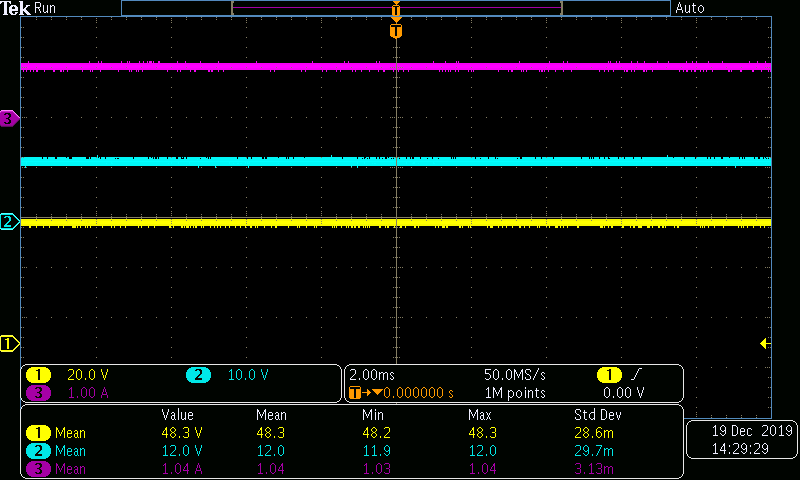
\includegraphics[width=0.8\textwidth]{graphics/Eingan_Ausgang_Strom_12V.png}
	\caption{Messung der Ausgangsspannung bei einem Laststrom von 1A} 
	\label{fig:Eingan_Ausgang_Strom_12V}
\end{figure}

Folgende Spannungen und Ströme sind in Abbildung \ref{fig:Eingan_Ausgang_Strom_12V} zu sehen: 

\begin{itemize}
	\item 1 Eingangsspannung (gelb)
	\item 2 Ausgangsspannung (blau)
	\item 3 Ausgangsstrom (violett)
\end{itemize}
 
Wie man erkennen kann, wird die Ausgangsspannung sauber auf 12V geregelt. Diese bleibt auch unter grösserer Belastung stabil. Die Testkondition wurde bewusst auf 1A Ausgangsstrom gesetzt, da die Pumpen diesen Strom niemals erreichen können. Somit ist sichergestellt, dass die Funktion der Speisung voll umfänglich gewährleistet ist.

Der Schaltregeler taktet die Spule gemäss Datenblatt mit einer Frequenz von ca. 100kHz. Um dies auszumessen, wurde die getaktete Spannung an V$_{sw}$ ausgemessen. Dies ist in Abbildung \ref{fig:Taktfrequenz_12V} zu sehen. 

\begin{figure}[h!]
	\centering
	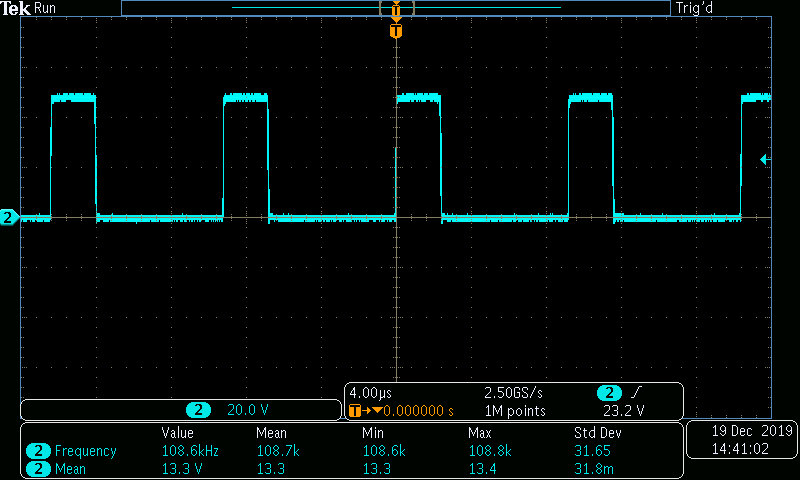
\includegraphics[width=0.8\textwidth]{graphics/Schaltfrequenz_SW_12V.png}
	\caption{Messung der Schaltfrequenz des 12V Reglers} 
	\label{fig:Taktfrequenz_12V}
\end{figure}

Die Taktfrequenz liegt wie erwartet bei ca. 100kHz. Bei der Messung ergab sich eine Schaltfrequenz von 108.6kHz.

\subsubsection{5V Speisung}\label{subsubsec:Hardware_Verifikation_5V_Speisunge}

Bei der 5V Speisung handelt es sich gemäss Kapitel \ref{subsubsec:5V_Speisung} fast exakt um den selben Aufbau, wie bei der 12V Speisung. Diese wird jedoch bei weitem nicht so stark belastet wie die 12V Speisung. Trozdem wurde auch diese Speisung bei einem Laststom von ca. 1A ausgemessen. In Abbildung \ref{fig:Eingang_Ausgang_Strom_5V} kann die Ausgangsspannung begutachtet werden.

\begin{figure}[h!]
	\centering
	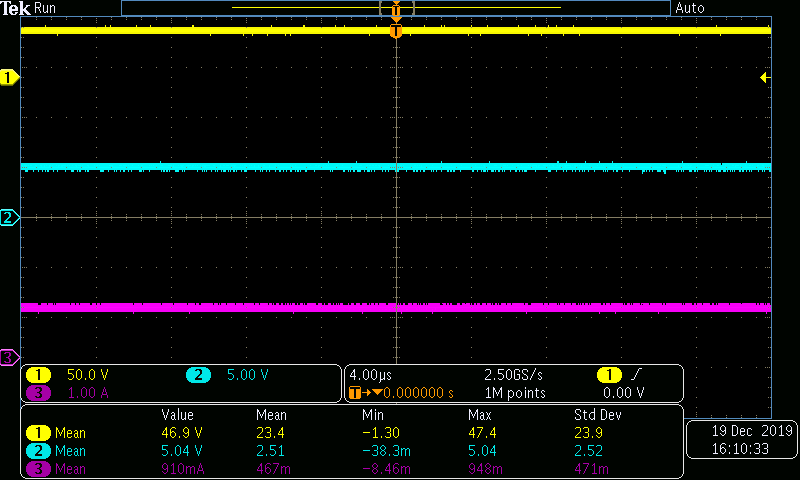
\includegraphics[width=0.8\textwidth]{graphics/Eingang_Ausgang_Strom_5V.png}
	\caption{Messung der Ausgangsspannung bei einem Laststrom von 1A} 
	\label{fig:Eingang_Ausgang_Strom_5V}
\end{figure}
\newpage
Folgende Spannungen und Ströme sind in Abbildung \ref{fig:Eingang_Ausgang_Strom_5V} zu sehen: 

\begin{itemize}
	\item 1 Eingangsspannung (gelb)
	\item 2 Ausgangsspannung (blau)
	\item 3 Ausgangsstrom (violett)
\end{itemize}

Auch bei der 5V Speisung wird die Ausgangsspannung erwartungsgemäss und zuverlässig auf 5V geregelt. Um die Schaltfrequenz des Reglers zu überprüfen, wurde auch hier wieder V$_{sw}$ ausgemessen. Dies ist in Abbildung \ref{fig:Taktfrequenz_5V} zu sehen.

\begin{figure}[h!]
	\centering
	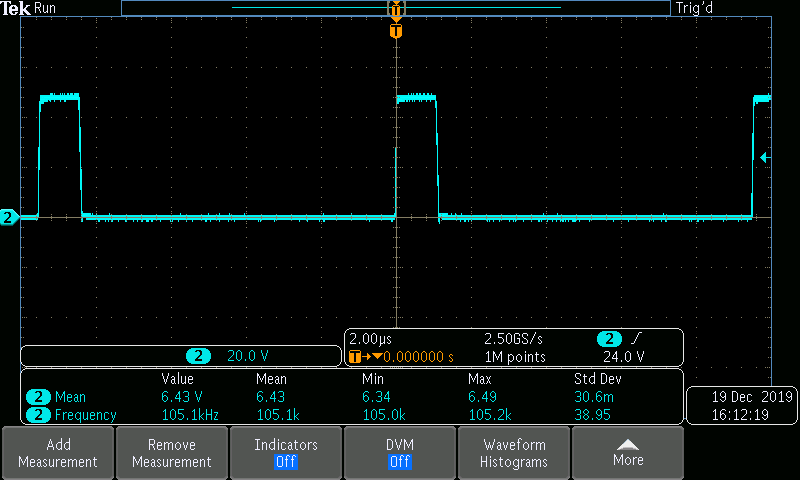
\includegraphics[width=0.8\textwidth]{graphics/Schaltfrequenz_SW_5V.png}
	\caption{Messung der Schaltfrequenz des 5V Reglers} 
	\label{fig:Taktfrequenz_5V}
\end{figure}

Auch hier wurde die Erwartung von ca. 100kHz erfüllt. Die Messung ergab eine Schaltfrequenz von 105.1kHz.